% Tipo de documento
% ***********************************************
% ***********************************************
\documentclass[xcolor=table]{beamer} %[draft]

% No lo he trabajado bien
% ***********************************************
%\usepackage{handoutWithNotes}
%\pgfpagesuselayout{2 on 1 with notes landscape}[a4paper,border shrink=5mm]

% Cargando paquetes
% ***********************************************
\usepackage[english]{babel}
%\usepackage[latin1]{inputenc}
%\usepackage[spanish, activeacute]{babel}
%\usepackage[spanish]{babel}
\usepackage[utf8]{inputenc}

%Juan Carlos Vergara Gallego
%%%%%\documentclass{beamer}
\usepackage{hyperref}
\usepackage{subfig}  %% Para incluir subgraficos
\usepackage{graphicx}
\usepackage{media9} % 
\usepackage{url}
\usepackage{ragged2e}  % Allow justification
\usepackage[margin=20pt,font=small,labelfont=bf,labelsep=period]{caption}


% Templates beamers
% ***********************************************
\usetheme[compress]{Dresden}
%\usecolortheme{dolphin}
\setbeamercovered{transparent}
%\usefonttheme[onlymath]{serif}
\usefonttheme[onlysmall]{structurebold}
%\usefonttheme{serif}
\beamertemplatenavigationsymbolsempty
\useinnertheme[shadow=true]{rounded}


% Más paquetes
% ***********************************************
\usepackage{color}
\usepackage{colortbl}
\usepackage{ziffer}
\usepackage{amsmath, amssymb}
\usepackage{etex}
\usepackage[absolute,overlay]{textpos}
\usepackage{framed}
\usepackage{multimedia}

\usepackage{decimal}
\usefonttheme{serif}  % Make equations to be in serif fonts
%\decimalpoint


\hypersetup{pdfstartview={Fit}, bookmarks=True, pdftitle={SCEC Presentation}, pdfauthor={Juan Carlos Vergara-Gallego}, pdfsubject={Presentation}, pdfkeywords={Waves, Elasticity, Numerical Methods, High Performance Computing, BEM}, pdfpagemode=UseOutlines, bookmarks, bookmarksopen, pdfstartview=FitH, colorlinks,linkcolor=blue, urlcolor=black, citecolor=blue}  % Configure hyperref

%--- New commands ----%
\newcommand{\footref}[1]{\textsuperscript{\ref{#1}}}
\newcommand{\pardiff}[2]{\frac{\partial #1}{\partial #2}}
\newcommand{\pardiffd}[2]{\frac{\partial^2 #1}{\partial #2^2}}




% Definitions
% ***********************************************
\setlength{\TPVertModule}{\paperheight}
\setlength{\TPHorizModule}{\paperwidth} 
\setlength{\TPHorizModule}{\paperwidth}\setlength{\TPVertModule}{\paperheight}

\setbeamercolor{footlinecolor}{bg=grayJuan,fg=blueEAFIT}
%\setbeamercolor{footlinecolor}{bg=yellowEAFIT,fg=blueEAFIT} %Define el color de la banda inferior


% Información que va en la franja inferior
%sep: define el alto de la franja inferior
\setbeamertemplate{footline}{%
  \begin{beamercolorbox}[sep=.15em, wd=\paperwidth,leftskip=0.4cm,rightskip=0.4cm]{footlinecolor}
  \mbox{
	\begin{minipage}{0.2\paperwidth}
		
\includegraphics[width=0.1\paperwidth]{img/logo.pdf}
	\end{minipage}
	\begin{minipage}{0.7\paperwidth}
		\begin{center}
			Juan Carlos Vergara Gallego. -- Mecánica Aplicada
		\end{center}
	\end{minipage}
	\begin{minipage}{0.1\paperwidth}
		\scriptsize{\insertframenumber}
	\end{minipage}}
  \end{beamercolorbox}%
}


% Definiendo los colores
% ***********************************************
\definecolor{grayJuan}   {HTML}{e6e4e4}
%\definecolor{blueEAFIT}   {HTML}{003560}
\definecolor{grenJuan}  {HTML}{94c11c}
\definecolor{middlegray}{rgb} {0.5,0.5,0.5}
\definecolor{lightgray} {rgb} {0.97,0.97,0.97}
\definecolor{tablegray} {rgb} {0.85,0.85,0.85}
\definecolor{white}     {rgb} {1.0,1.0,1.0}
\definecolor{orange}    {rgb} {0.8,0.3,0.3}
\definecolor{jac}       {rgb} {0.6,0.6,0.1}
\definecolor{red}       {rgb} {1.0,0,0}
\definecolor{green}     {rgb} {0.0,1.0,0.0}
\definecolor{black}     {rgb} {0,0,0}
\definecolor{blue}      {rgb} {0,0,1.0}
\definecolor{lightblue} {rgb} {0.5,0.9,1.0}
\definecolor{yellowEAFIT} {rgb} {1,.725490196,.011764705} %Adicionado por Juan Para que Case con el color amarillo de Eafit
\definecolor{blueEAFIT}   {rgb}{0, 0.294117647, 0.521568627} %Adicionado por Juan Para que Case con el color azul de Eafit

% Configuración colores diapositivas
% ***********************************************
\setbeamercolor{block body example}{bg=grayJuan}
\setbeamercolor{block title example}{bg=blueEAFIT,fg=white}
\setbeamercolor{block body alerted}{bg=grayJuan}
\setbeamercolor{block title alerted}{bg=red,fg=black}

\setbeamercolor{section in head/foot}{fg=white, bg=yellowEAFIT} %Modifica el color de la franja superior
\setbeamercolor{subsection in head/foot}{fg=black, bg=blueEAFIT} %Modifica el color de la segunda franja superior
%\setbeamercolor{normal text}{fg=blueEAFIT}
\setbeamercolor{block title}{fg=blueEAFIT}
\setbeamercolor{section in toc}{fg=blueEAFIT}
\setbeamercolor{section}{fg=blueEAFIT}
\setbeamercolor{item}{fg=blueEAFIT} %Determina el color de los circulos cuando se usa el comando item
%\setbeamercolor{frametitle}{fg=blueEAFIT,bg=grayJuan}
\setbeamercolor{frametitle}{fg=blueEAFIT,bg=grayJuan}%Esta linea determina el color de la tercera franja superior
\setbeamercolor{framesubetitle}{fg=black}
\setbeamercolor{title}{fg=blueEAFIT,bg=grayJuan} %Controla el color del título
\setbeamercolor{titlelike}{bg=blueEAFIT}
%\setbeamercolor{fine separation line}{}
%\setbeamercolor{frametitle}{fg=black}
%\setbeamercolor{item projected}{fg=white}
%\setbeamercolor{normal text}{bg=white,fg=black}
\setbeamercolor{palette sidebar primary}{use=normal text,fg=normal text.fg}
\setbeamercolor{palette sidebar quaternary}{use=structure,fg=structure.fg}
\setbeamercolor{palette sidebar secondary}{use=structure,fg=structure.fg}
\setbeamercolor{palette sidebar tertiary}{use=normal text,fg=normal text.fg}

\setbeamercolor{section in sidebar}{fg=grayJuan}%Juan
\setbeamercolor{section in sidebar shaded}{fg=grayJuan}
\setbeamercolor{separation line}{}
\setbeamercolor{sidebar}{bg=grayJuan}
\setbeamercolor{sidebar}{parent=palette primary}
%\setbeamercolor{section in sidebar}{fg=grayJuan}
%\setbeamercolor{section in sidebar shaded}{fg=grayJuan}
%\setbeamercolor{separation line}{}
%\setbeamercolor{sidebar}{bg=grayJuan}
%\setbeamercolor{sidebar}{parent=palette primary}

%\setbeamercolor{structure}{bg=grenJuan, fg=blueEAFIT}

% Organizando la primer página, donde va el título
% ***********************************************
\setbeamertemplate{title page}{
	\vspace{-0.25cm}
	
\includegraphics[height=1cm]{img/logo.pdf}\\
	\vspace{0.5cm}
        \begin{columns}
        \column{.5\textwidth}
        	  \insertsubtitle\\
	  \vspace{0.5cm}
	  {\usebeamerfont{title}\usebeamercolor[fg]{title}\inserttitle}\\
	  \vspace{0.5cm}
	  \insertauthor\\
	  \insertdate
	  \vfill
        \column{.5\textwidth}
	\begin{center}
	  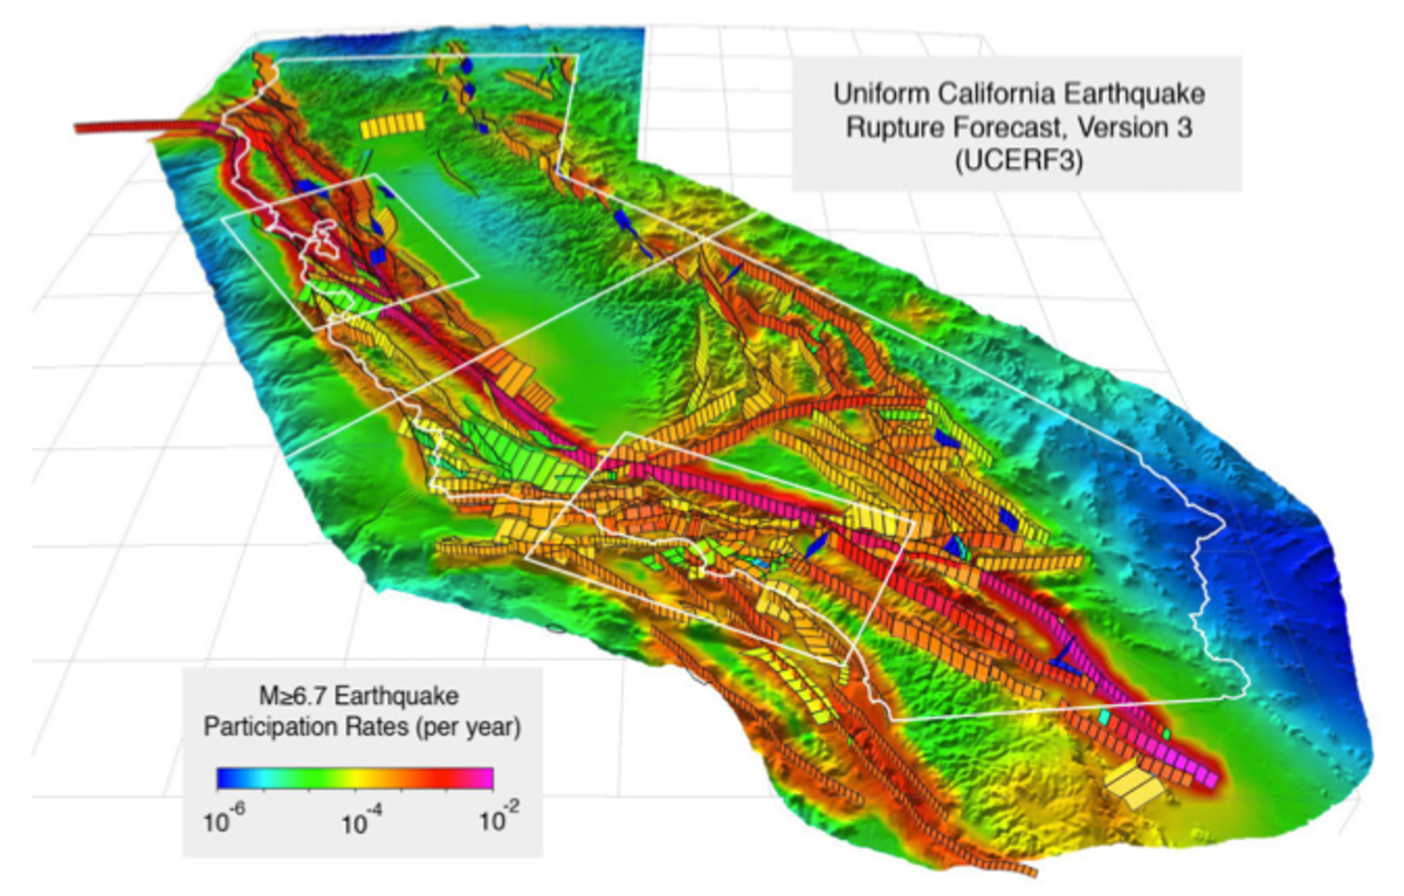
\includegraphics[width=1\textwidth]{img/UCERF3_Map.pdf}
	\end{center}
 \end{columns}	

}

%\decimalpoint